% Author: Izaak Neutelings (October 2020)
% Inspiration: https://tex.stackexchange.com/questions/25531/adding-underbrace-in-tikz
\documentclass[border=3pt,tikz]{standalone}
\usepackage{physics}
\usepackage{siunitx}
\usepackage{ifthen}
\usepackage{tikz}
%\usepackage[outline]{contour} % glow around text
\usetikzlibrary{calc}
\usetikzlibrary{angles,quotes} % for pic
\usetikzlibrary{patterns}
\tikzset{>=latex} % for LaTeX arrow head
%\contourlength{1.4pt}

\colorlet{xcol}{blue!70!black}
\colorlet{vcol}{green!70!black}
\colorlet{myred}{red!65!black}
\colorlet{acol}{red!50!blue!80!black!80}
\tikzstyle{ground}=[preaction={fill,top color=black!10,bottom color=black!5,shading angle=20},
                    fill,pattern=north east lines,draw=none,minimum width=0.3,minimum height=0.6]
\tikzstyle{metal}=[fill,top color=black!40,bottom color=black!20,shading angle=10]
\tikzstyle{mass}=[line width=0.6,red!30!black,fill=red!40!black!10,rounded corners=1,
                  top color=red!40!black!20,bottom color=red!40!black!10,shading angle=20]
\tikzstyle{rope}=[brown!70!black,very thick,line cap=round]
\def\rope#1{ \draw[black,line width=1.5] #1; \draw[rope] #1; }

% FORCES SWITCH
\tikzstyle{force}=[->,myred,very thick,line cap=round]
\tikzstyle{Fproj}=[force,myred!40]
\newcommand{\vbF}{\vb{F}}
\newcommand{\vbT}{\vb{T}}

\begin{document}

% CIRCULAR MOTION - 2D
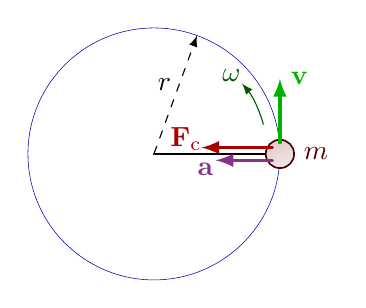
\begin{tikzpicture}
    \def\R{1.6}  % string length
    \def\r{0.18} % ball radius
    \def\Ry{0.5} % small radius of the ellipse
    \def\F{0.9}  % force size
    \coordinate (O) at (0,0);
    \coordinate (M) at (\R,0);
    \coordinate (F0) at ($(M)+(104:0.8*\r)$);
    \coordinate (F) at ($(F0)+(90:\F)$);
    \draw[very thin,xcol] (O) circle (\R);
    \draw[->,dashed] (O) -- (70:\R) node[midway,above left=-2] {$r$};
    \draw[thick,line cap=round] (O) -- (\R,0); %node[midway,above left=-2] {$r$};
    \draw[thin,mass] (M) circle (\r) node[right=5] {$m$};
    \draw[force] (M)++(140:0.7*\r) --++ (-\F,0) node[below=1,above left=-4] {$\vb{F}_\mathrm{c}$};
    \draw[force,acol] (M)++(-140:0.7*\r) --++ (-0.8*\F,0) node[below left=-3] {$\vb{a}$};
    \draw[force,vcol] (M)++(90:0.8*\r) --++ (0,0.9*\F) node[right=0] {$\vb{v}$};
    \draw[->,vcol!50!black] (15:0.9*\R) arc(15:40:0.85*\R) node[above left=-3] {$\omega$};
\end{tikzpicture}


\end{document}